\documentclass[11pt]{article}
\usepackage[utf8]{inputenc}
\usepackage{amsmath, amsthm, amssymb}
\usepackage{graphicx}
\author{Fabian Alenius, Kjell Winblad and Chongyang Sun} \title{Handwritten Text Recgonition}
\begin{document}
\maketitle

\begin{abstract}
Hello.

\end{abstract}

\section{Introduction}
%1. Give general introduction to area.
%2. Describe why it's important.
%3. Applications.
%4. Contributions.

%Fabian
\section{Introduction}

Recognition of handwritten text has been a popular research area for decades because it can be used in so many different applications.
Formally, handwritten recognition is the task of transforming a language represented in graphical form into its symbolic representation \cite{introsurvey}.
There are two different approaches to handwritten recognition, \textit{online} and \textit{offline}.
In the online approach we know the order in which the strokes and individual points were drawn.
This information can easily be captured if the text is recorded by a digital pen or on a touchscreen.
In the offline approach we are only given the final image.
Online recognition is primarily used for signature verification, author authentication and digital pens.
Application areas for offline recognition include postal automation, bank cheque processing and automatic data entry \cite{intro1}.
In this paper we only consider offline handwritten recognition.

The ultimate goal in handwritten recognition is to recognize words.
However, one way to potentially decompose or simplify the problem is to segment words into its individual characters \cite{intro-Yacoubi}. 
Segmentation can either be done \textit{explicitly} or \textit{implicitly}.
Explicit segmentation tries to separate the word at character boundaries while implicit segmentation separates the word into equal sized frames.
The implicit frames, each represented by a feature vector, are then mapped into characters.

\section{Previous work}
Because handwritten recognition is such a well-researched area there is a wealth of literature available.
We mention only a few references that we found helpful.
Cheriet et al. \cite{Cheriet} gives a good review of the development of handwritten recognition.
They also go on to give a broad overview of feature extraction and classification using a plethora of different techniques.
Rabiner, L. R. \cite{Rabiner1989} gives an excellent review of Hidden Markov Models (HMM) and the Baum-Welch training algorithm, as well as how to apply them in speech recognition.
El-Yacoubi et al. \cite{intro-Yacoubi} introduce an approach to recognize text using Hidden Markov Models with explicit word segmentation.
Laan et al. \cite{initialmodel} covers different initial model selection techniques for the Baum-Welch algorithm.
Despite impressive progress over the last couple of decades, performance is still far away from human performance.




\section{Previous work}
%Write about other papers and how they have solved the problem.

\section{Problem}\label{sec:problem}
%Describe our limited version of the problem.
%Describe the two problems, one is recognizing characters and the other is to recognize words.
%1. Images have strokes of width 1.
%2. Assume characters segment in word.

\section{Method}\label{sec:method}

This section describes the handwritten text recognition system. It starts by giving a top level overview of the system and then it describes the details such as the HMM implementation, feature extraction and the datasets used for training. 

%2. General overview of our implementation.   Kjell
%	Two classifiers
%		What they are doing
%3. Add picture describing implementation.  Kjell

\subsection{General Overview of Classifiers}\label{sec:overview_of_classifiers}


The handwriting recognition system has two levels, each containing a classifier. 
The first classifier is a function that takes an image as input and outputs a character. 
The second classifier is a function that takes a string of characters as input and outputs a word.

We have implemented two kinds of word classifiers.
The first one called the \emph{Forward-classifier} has exactly the same architecture as the character classifier and is explained in this section.
The second one is called \emph{Viterbi-classifier} and is explained in Section~\ref{sec:word_classifiers}.
A flowchart that shows the classification process can be seen in Figure~\ref{fig:classification_system_overview}. 

    \begin{figure}[htb] 
      \begin{center}
	\leavevmode
	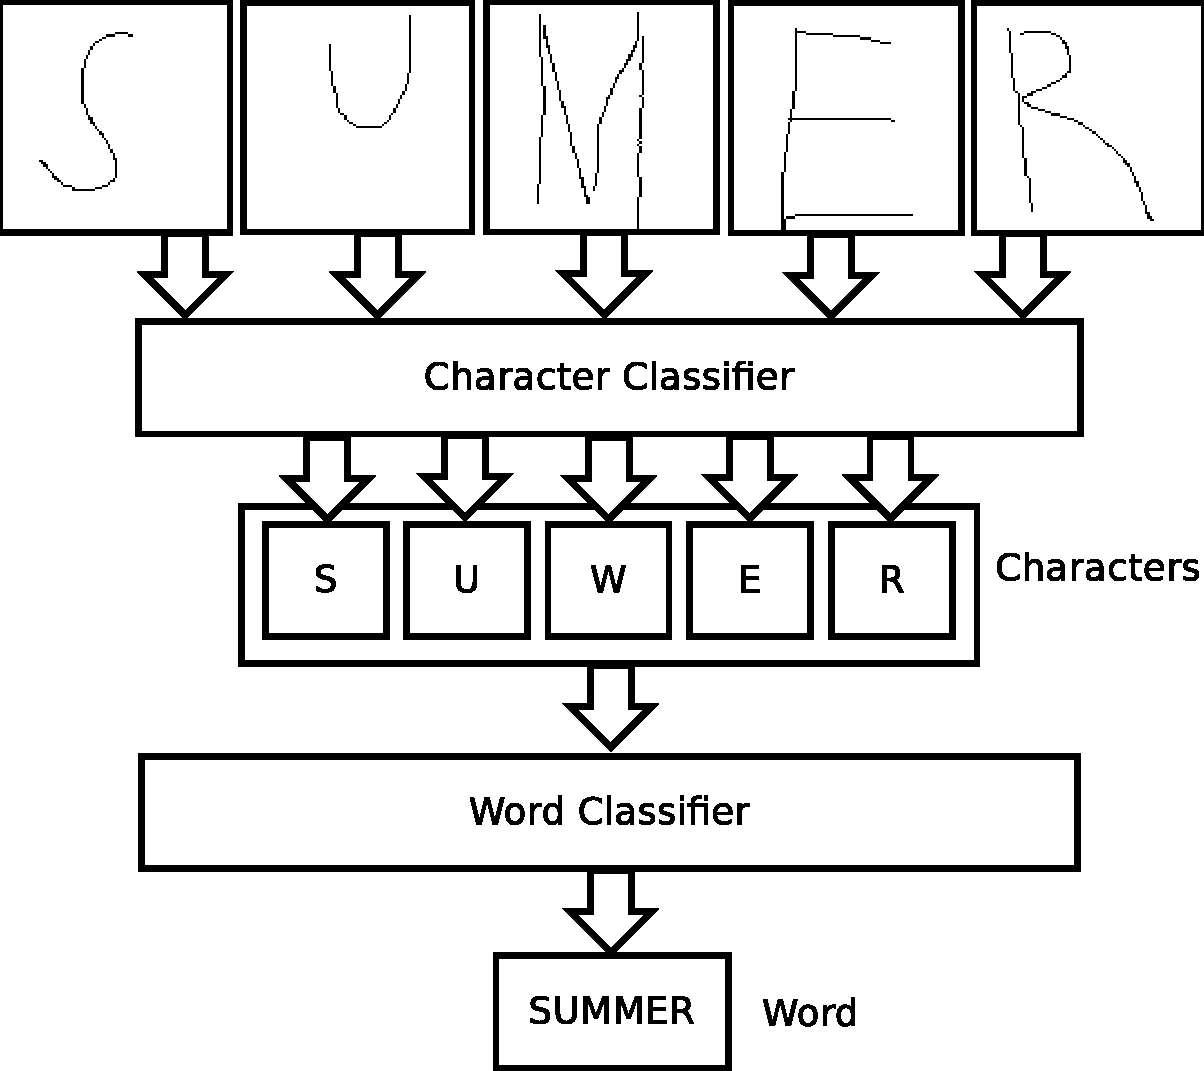
\includegraphics[width=110mm]{classification_system_overview.pdf}%width=115mm,height=40mm
      \end{center}
      \caption{Flowchart of classification process.}
      \label{fig:classification_system_overview}
    \end{figure}

The classifiers contain HMMs for all elements in the set of possible outputs. 
So if the character classifier is trained to recognize the 26 Latin characters, it will contain 26 HMMs. 
When the classifiers are trained they are given input examples for all possible outputs. 
If the input $I$ is given to one of the classifiers the following steps are performed to calculate the output:

\begin{enumerate}
  \item The probability of $I$ is calculated for all HMMs contained in the classifier:
    \begin{enumerate}
      \item $I$ is translated into a sequence of observation symbols $\mathbf{O} = O_{1},O_{2},...,O_{n}$. 
      If $I$ is a string of characters and the output of the classifier is a word, the translation is straightforward. 
      Every character in the string is simply translated to the corresponding observation symbol. 
      There are also special observations for the start and end states. 
      This is explained in more detail in the following sections. 
      If $I$ is an image, the image is first segmented to a sequence of segments. 
      An observation symbol is then obtained from all segments. 
      See section~\ref{sec:image-preprocessing} for more information about the image feature extraction.
      \item The Forward algorithm \cite{Rabiner1989} is then used to calculate the probability of $\mathbf{O}$ given the HMM.
    \end{enumerate}
  \item The output symbol with the highest probability in the previous step is returned as output.
\end{enumerate}
 
 %% I think this sentence should be split up or turned into a list. It's hard to read in its current form imo. --Fabian
The following parameters must be supplied when a classifier is created\footnote{A few more parameters can be given but are not listed here because of lack of importance. See the source code of the system for information about other parameters. How the source code can be obtained is explained in appendix~\ref{app:source_code}.}:
\begin{itemize}
 \item The set of possible output symbols and corresponding training examples.
 \item The initialization method that should be used by the HMMs.
 \item A binary variable, specifying if the training examples should be used to train the model with the Baum-Welch \cite{Rabiner1989} training algorithm.
\end{itemize}


%1. Describe HMM, short overview. Chongyang
%1 Picture of HMM topology
%4. Describe the different initialization algos, advantages and disadvantages. Chongyang
%1.1Topology of HMM Chongyang
%1.2 prevention of underflow. Chongyang
%1.3 Handle zeros in denominator. Chongyang 




\subsection{Datasets}\label{sec:dataset}
%1. Write about creation of sample data. Chongyang
%2. Could not find good dataset. Chongyang
%3. Write down how much data we had. Chongyang
%4. Write about how the word examples are generated

\subsection{Image Preprocessing and Feature Extraction}\label{sec:image_preprocessing}
%1. Write about scaling of picture. Kjell
%2. Segmentation of picture. Kjell

The character classifier classifies images with handwritten characters as described in section~\ref{sec:overview_of_classifiers}. A sequence of observation symbols is extracted from the images given as training data and when an image shall be classified. This process is called feature extraction. As mentioned in section~\ref{sec:problem}, our system assume that there is one image per character, that the lines in the characters are of a single color and the width of the lines have width one. The feature extraction process can be divided into the following steps:

\begin{enumerate}
  \item The scaling step makes sure that the character fills the whole images. Because of this step, it does not matter where in the given image the character is painted. The scaling may have the problem that the lines are getting thicker than one pixel after scaling if the original painted character just fills a small part of the image\footnote{The standard Java image scaling algorithm is used for the scaling.}. This problem will be handled in some sense if the training examples contains images where the character fills a small part of the image. The following algorithm is used to the scaling:
  \begin{enumerate}
    \item The minimum rectangle $R$ in the image that contains the whole character is found.
    \item The rectangle $R$ is scaled to fill the size of the original picture. The scaled version of $R$ is returned as the scaled image.
  \end{enumerate}
  \item The new scaled image is sliced into $N$ vertical segments of the same since.
  \item An observation symbol is extracted from every segment in the following way:
  \begin{enumerate}
    \item The number of pixels in the three largest components in the segment are found and put into a triple $(s_{1},s_{2},s_{3})$ which is sorted so the largest number is first. A component is defined as a set of colored pixels that are connected and that contains all pixels that are connected to one of the pixels in the set. Two colored pixels are connected if they are neighbors or if it is possible two create a path of colored connected pixels between them. All pixels except the border pixels have 8 neighbors. If the segment contains less than three components, the triple is filled with zeros.
    \item The elements in the triple is classified to one be $Large$, $Small$ or $None$. The classification function $c$ is defined as in equation~\ref{eq:classification_function}.
    \begin{equation}\label{eq:classification_function}
    c(s) = None \text{ if } s = 0, Large \text{ if } s > d \text{ and } Small \text{ otherwise}
    \end{equation}, where $d$ is a classification constant. The triple $(s_{1},s_{2},s_{3})$ is translated to a triple of classes $(c_{1},c_{2},c_{3})$ by applying the function $c$ to all elements of the triple.
    \item The triple of classes is mapped to an observation symbol. The mapping is defined by the set of relations that can be found in equation~\ref{eq:class_triple_to_observation_symbol_mappings}.

    \begin{equation}\label{eq:class_triple_to_observation_symbol_mappings}
     \substack{ LLL\rightarrow a,LLS\rightarrow b,LSS\rightarrow c,LSN\rightarrow d,LLN\rightarrow e,LNN\rightarrow f,\\
    SSS\rightarrow g,SSN\rightarrow h,SNN\rightarrow i,NNN,\rightarrow j }
    \end{equation}
    , where $LSN$ is a short form of $(Large,Small,None)$ and so on.
  \end{enumerate}  
\end{enumerate}

The classification constant $c$ and the number of segments $N$ are parameters to the feature extractor. An example of feature extraction for an image can be seen in figure~\ref{fig:image_feature_extraction}.

%    \begin{figure}[htb] 
%      \begin{center}
%	\leavevmode
%	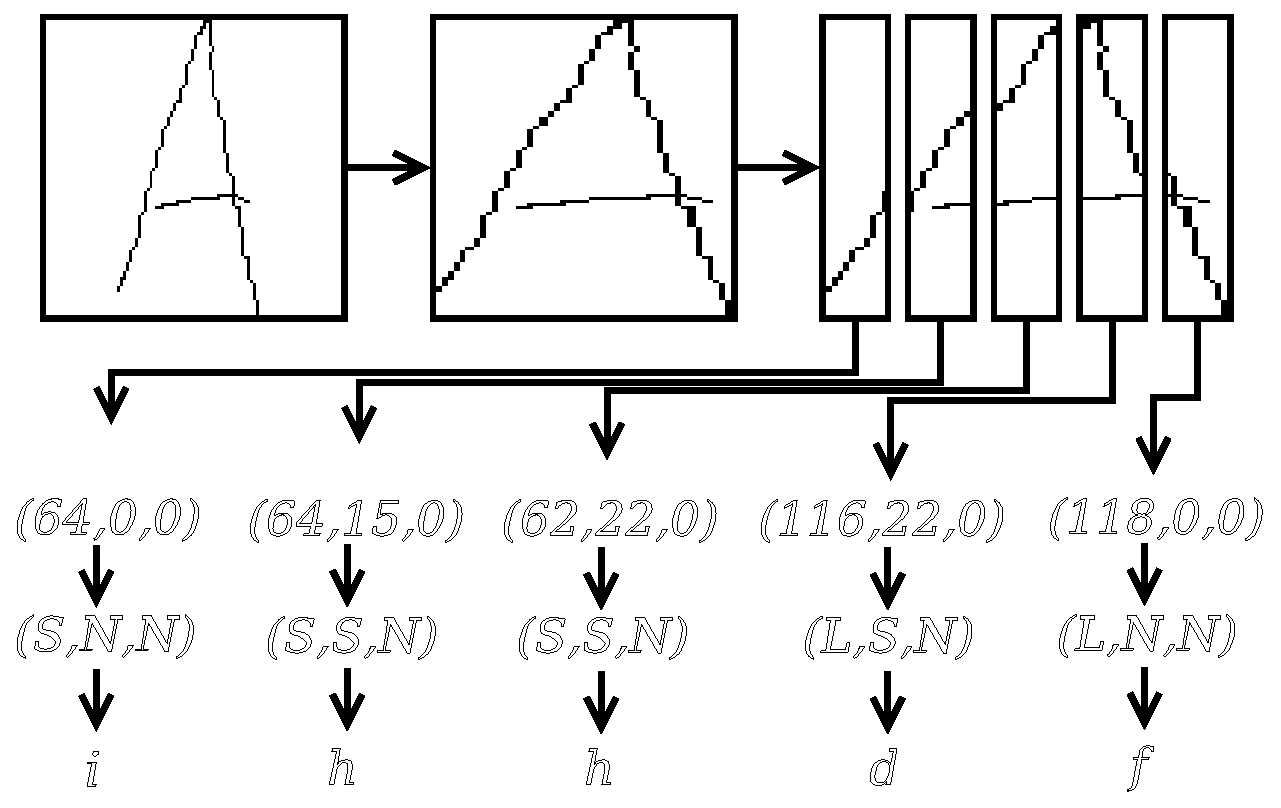
\includegraphics[width=110mm]{image_feature_extraction.eps}%width=115mm,height=40mm
%      \end{center}
%      \caption{Example of image feature extraction.}
%      \label{fig:image_feature_extraction}
%    \end{figure} 

\section{Result}\label{sec:result}
%1. (Started Kjell) Test of different initialization methods and number of training examples for word recognition 
%1. (Started Kjell) Test of different initialization methods and number of training examples for word recognition
%1. Maybe result from character test using different initialization algos.
%2. Basic results from testing the implementation
%3. Better to do in appendix? Depending on how much other results we have, discuss experience of playing around with the gui.

\subsection{Word Classifier and Different Initialization Methods}\label{sec:word_classifier_results}

In this section classification results for the words in Table~\ref{tab:words_supported_by_classifier} will be presented. 
See section~\ref{sec:method} for a description of the implementation of the classifiers.
The training and test example words were randomly generated with the generator having the properties in Table~\ref{tab:word_generator_properties}.
See section~\ref{sec:dataset}, for more information about the word example generator. 
To test the accuracy of the created classifiers, 100 test examples were used. 
Five test examples for every word. 
The test examples were generated using the same properties as the training examples.
Two initialization methods, count based initialization and random initialization, were tested with 100, 200, 400, 800 and 1600 training examples. 
The results of the test is presented in Table~\ref{tab:word_classifier_results_generated_data}. 
It contains the test scores for the two initialization methods before and after training with the Baum-Welch algorithm. 
The test score is defined as the percentage of correctly classified test examples.

\begin{table}[htb]
  \begin{center}
  \begin{tabular}{ l l l l l }
    dog      & cat       & pig     & love       & hate  \\
    scala    & python    & summer  & winter     & night  \\ 
    daydream & nightmare & animal  & happiness  & sadness \\ 
    tennis   & feminism  & fascism & socialism  & capitalism \\
  \end{tabular}
\end{center}
\caption{Words supported by the resulting classifier.} 
\label{tab:words_supported_by_classifier} 
\end{table}

\begin{table}[htb]
  \begin{center}
  \begin{tabular}{ l l }
    Probability of extra letter at position         & 0.03 \\
    Probability of extra letter equal neighbor      & 0.7 \\ 
    Probability of wrong letter at position         & 0.1 \\ 
    Probability of letter missing at position       & 0.03 \\
  \end{tabular}
\end{center}
\caption{Properties obeyed by the word training example generator.} 
\label{tab:word_generator_properties} 
\end{table}

\begin{table}[htb]
  \begin{center}
  \begin{tabular}{ l l l l l l l }
    NOE    & RIBF   & CBIBT  & RIAT    & CBIAT  & RITT & CBITT\\ \hline
    $100$  & $3$ & $99$   & $1$     & $0$    & $6$  & $3$\\ 
    $200$  & $2$ & $100$  & $13$    & $36$   & $12$ & $5$\\ 
    $400$  & $2$ & $100$  & $90$    & $95$   & $23$ & $7$\\
    $800$  & $1$ & $100$  & $100$   & $100$  & $46$ & $13$\\   
    $1600$ & $5$ & $100$  & $100$   & $100$  & $96$ & $26$\\  
  \end{tabular}
\end{center}
\caption{Test with different number of training examples and different initialization methods.
	 NOE=''number of training examples for every word'',
         RIBF=''random initialization score before training'',
         CBIBT=''count based initialization score before training'',
         RIAT=''random initialization score after training'',
         CBIAT=''count based initialization score after training'',
         RITT=''random initialization training time (minutes)'',
         CBITT=''count based initialization training time (minutes)''} 
\label{tab:word_classifier_results_generated_data} 
\end{table}

\subsection{Character Classification with Different Parameters}\label{sec:character_classifier_results}

As described in section~\ref{sec:image_preprocessing} the image feature extraction step in the character classifier takes two parameters.
The first parameter is the number of segments that shall be created. 
The second parameter is the size classification factor which is used in equation~\ref{eq:classification_function}. 
For the experiment we only had 100 examples for each of the 26 characters. 
How the examples are produced is described in section~\ref{sec:dataset}. 
An initial experiment was performed to test count based initialization and random initialization before and after training with the Baum-Welch algorithm.
The initial experiment shows that there is probably too few training examples for the training to have any positive effect for count based initialization. 
This could possible be fixed to some extend with some kind of smoothening of the model produced by the training. 
10 test examples and 90 training examples for every character were selected randomly from the example set for the experiments. 
The results from the initial experiment can be found in table~\ref{tab:character_classifier_initial_experiment}. 
In the initial experiment $1.3$ was used as the size classification factor and the number of segments was set to $7$.


\begin{table}[htb]
  \begin{center}
  \begin{tabular}{ l l l l l }
    NOE    & RIBF   & CBIBT  & RIAT    & CBIAT \\ \hline
    $90$  & $4$ & $53$ & $16$  & $16$  \\   
  \end{tabular}
\end{center}
\caption{Test of the character classifier with different initialization methods and before and after training.
	 NOE=''number of training examples for every word'',
         RIBF=''random initialization score before training'',
         CBIBT=''count based initialization score before training'',
         RIAT=''random initialization score after training'',
         CBIAT=''count based initialization score after training''} 
\label{tab:character_classifier_initial_experiment} 
\end{table}

Only count based initialization is looked upon in the experiment of different parameters, because the initial experiment showed that the best result seems to be produced when just using count based initialization and no training.
When testing the parameters, 5 models were created in the same way as in the initial experiment. 
The average accuracy for these 5 models when testing them with their own test example set was recorded as the accuracy for the configuration. 
For all 5 models that were created, different training example sets and test example sets were randomly selected. 
90 training examples and 10 test examples were used for every character as in the initial experiment. 
The results of the experiment can be seen in table~\ref{tab:character_classifier_results_different_parameters}.

\begin{table}[htb]
  \begin{center}
  \begin{tabular}{ c | l l l l l l l l l }
CCF\textbackslash NOS &    4   & 5      & 6      & 7      & 8      & 9      & 10     & 11     & 12 \\ \hline
0.7     &  $32$  &  $38$  &  $43$  &  $42$  &  $44$  &  $44$  &  $45$  &  $48$  &  $48$  \\
1.0     &  $35$  &  $39$  &  $42$  &  $41$  &  $44$  &  $49$  &  $48$  &  $47$  &  $48$  \\
1.3     &  $43$  &  $47$  &  $53$  &  $53$  &  $53$  &  $56$  &  $57$  &  $56$  &  $59$  \\
1.6     &  $47$  &  $49$  &  $53$  &  $55$  &  $57$  &  $57$  &  $58$  &  $57$  &  $57$  \\
1.9     &  $50$  &  $52$  &  $56$  &  $57$  &  $58$  &  $57$  &  $58$  &  $59$  &  $59$  \\
2.2     &  $55$  &  $57$  &  $60$  &  $60$  &  $62$  &  $62$  &  $62$  &  $65$  &  $63$  \\
2.5     &  $57$  &  $59$  &  $60$  &  $61$  &  $62$  &  $62$  &  $65$  &  $65$  &  $63$  \\
2.8     &  $55$  &  $60$  &  $61$  &  $62$  &  $64$  &  $65$  &  $66$  &  $64$  &  $65$  \\
3.1     &  $55$  &  $59$  &  $64$  &  $63$  &  $65$  &  $66$  &  $65$  &  $67$  &  $\textbf{68}$  \\
3.4     &  $56$  &  $60$  &  $62$  &  $64$  &  $64$  &  $65$  &  $65$  &  $67$  &  $65$  \\
3.7     &  $55$  &  $62$  &  $62$  &  $64$  &  $63$  &  $64$  &  $67$  &  $67$  &  $67$  \\
4.0     &  $56$  &  $61$  &  $61$  &  $65$  &  $64$  &  $64$  &  $66$  &  $66$  &  $65$  \\
4.3     &  $56$  &  $61$  &  $63$  &  $65$  &  $65$  &  $65$  &  $66$  &  $67$  &  $66$  \\
4.6     &  $55$  &  $60$  &  $62$  &  $65$  &  $65$  &  $65$  &  $67$  &  $\textbf{68}$  &  $66$  \\
4.9     &  $55$  &  $60$  &  $63$  &  $67$  &  $67$  &  $66$  &  $67$  &  $67$  &  $66$  \\
5.2     &  $54$  &  $60$  &  $63$  &  $65$  &  $64$  &  $67$  &  $66$  &  $65$  &  $65$  \\
5.5     &  $53$  &  $59$  &  $63$  &  $63$  &  $66$  &  $66$  &  $67$  &  $67$  &  $66$  \\
5.8     &  $51$  &  $60$  &  $63$  &  $65$  &  $63$  &  $67$  &  $68$  &  $66$  &  $66$  \\
  \end{tabular}
\end{center}
\caption{Results for character classification test with different parameters. The scores are percentage of correctly classified characters.
	 NOS=''number of segments'',
         CCF=''component classification factor''}
\label{tab:character_classifier_results_different_parameters} 
\end{table}


\section{Discussion}
%1. Discuss the results.
%2. Discuss importance of amount of training data and the effects on performance.
%3. Discuss possibility of training words with data from character classification
%4. Discuss how our approach might work for word recognition

\section{Future Work}
%1. Discuss what other test would be interesting to perform
%2. How can the classifier be improved. More features and real training data for the words?

\bibliographystyle{plain}	% (uses file "plain.bst")
\bibliography{myrefs}		% expects file "myrefs.bib"

\pagebreak

\appendix


\section{Source Code}\label{app:source_code}

The source code for the system described in this report can be found at the following address:

\begin{verbatim}
http://github.com/kjellwinblad/HandReco
\end{verbatim}

The source code can be downloaded as a ZIP-archive or cloned using git\footnote{http://git-scm.com/}.

\section{Result Reproduction}\label{app:result_reproduction} 

The test results presented in Section~\ref{sec:result} are produced by scripts written in the Jython\footnote{Jython is a version of Python for the Java Virtual Machine (http://www.jython.org/)} programming language. The following steps will run the test scripts:

\begin{enumerate}
 \item Follow the instructions in appendix~\ref{app:source_code} to download the source code for the system.
 \item Follow the instructions in the \verb|README.md| file in the root of the source code directory. These instructions will help you to set up your environment for running the test scripts.
 \item Open a system terminal and execute the following commands (Notice that the path may look different in your system):
 \begin{enumerate}
  \item \verb|cd /path/to/HandReco/src/test|
  \item To run tests for word classifier:
  \item \verb|jython word_classifer_tester.py|
  \item To run tests for character classifier:
  \item \verb|jython character_classifier_tester.py|
 \end{enumerate}
\end{enumerate}

\section{Testing Handwriting Recognition in Graphical User Interface}
%Kjell Describe the GUI for running the HandReco Writer and perhaps some comments on how it works
A graphical user interface (GUI) has been created in order to test the handwriting recognition system in practice. See Figure~\ref{fig:hand_reco_writer_screenshot} for a screenshot of the graphical user interface. The following steps can be used to run the GUI:

\begin{enumerate}
 \item Follow the instructions in appendix~\ref{app:result_reproduction} to step 2.
 \item Open a system terminal and execute the following commands (Notice that the path may look different in your system):
 \begin{enumerate}
  \item \verb|cd /path/to/HandReco/src/gui}|
  \item \verb|jython hand_reco_writer.py|
 \end{enumerate}
\end{enumerate}

The GUI can only recognize capital Latin letters. 
To see which words are available for word corrections click on the \textbf{Info$\Rightarrow$Available Words...} menu item. 
To input a character, first paint the character in the paint area and then press the \textbf{Write Character} button. 
To do a space, press the \textbf{Space} button. 
To do a space and let the word classifier correct the last word, press the \textbf{Space and Correct} button.

    \begin{figure}[htb] 
      \begin{center}
	\leavevmode
	\includegraphics[width=80mm]{Screenshot_HandReco_Writer.png}%width=115mm,height=40mm
      \end{center}
      \caption{Screenshot of HandReco Writer.}
      \label{fig:hand_reco_writer_screenshot}
    \end{figure}


\end{document}